% !TeX spellcheck = en_GB
\begin{figure}
  \setlength{\unitlength}{\textwidth}

        \begin{picture}(1,0.3)(-0.02,0)

      % % % Parkinson Data 
%      \put(0.025,0.5){\includegraphics[width=0.5\unitlength]{../FnP/gnuplot/displacement_amp_collapsed_parkinson.eps}}
%      \put(0.025,0.27){\includegraphics[width=0.5\unitlength]{../FnP/gnuplot/velocity_amp_collapsed_parkinson.eps}}
%      \put(0.495,0.27){\includegraphics[width=0.5\unitlength]{../FnP/gnuplot/velocity_amp_collapsed_re200.eps}}
      
      \put(0.025,0.02){\includegraphics[width=0.5\unitlength]{../FnP/gnuplot/mean_power_collapsed_parkinson.eps}}
      \put(0.495,0.02){\includegraphics[width=0.5\unitlength]{../FnP/gnuplot/mean_power_optimum_re_200.eps}}
%      \put(0.495,0.5){\includegraphics[width=0.5\unitlength]{../FnP/gnuplot/displacement_amp_collpased_re200.eps}}
      
%      \put(0.23,0.00){ $\displaystyle\frac{c}{\rho\mathcal{A}U}$}
%      \put(0.73,0.00){ $\displaystyle\frac{c}{\rho\mathcal{A}U}$}

      \put(0.28,0.00){\massdamp}
      \put(0.78,0.00){\massdamp}
      
     
       \put(-0.03,0.13){$\displaystyle\frac{P_{m}}{\rho \mathcal{A}U^3 }$}
      

      \put(0.095,0.217){\small(a)}
      \put(0.565,0.218){\small(b)}
      
    \end{picture}

  \caption{Mean power as a function of \massdamp. Data presented at (a) $\reynoldsnumber=22300$, $\massdamp=20000$ and (b) $\reynoldsnumber=200$, $\massdamp=100$. Hysteresis could be observed at high \reynoldsnumber  }
    \label{fig:collapsed_data}
\end{figure}

 %vspace{10cm}
